\section{Introducción}

Recientemente, se ha acrecentado el interés por los compuestos fluorescentes de boro debido a su amplio campo de aplicaciones; \autocite{ibarra-rodriguezOrganoboronSchiffBases2019} ya sea en sensores, como en tintas de seguridad, o bien los \gls{BODIPY} comercialmente disponibles utilizados como agentes para la tinción celular, ER-Tracker™ Green y ER-Tracker™ Red (ver \cref{ER-Trackers}).

\begin{scheme}[H]
	\centering
	\begin{subscheme}{0.45\linewidth}
		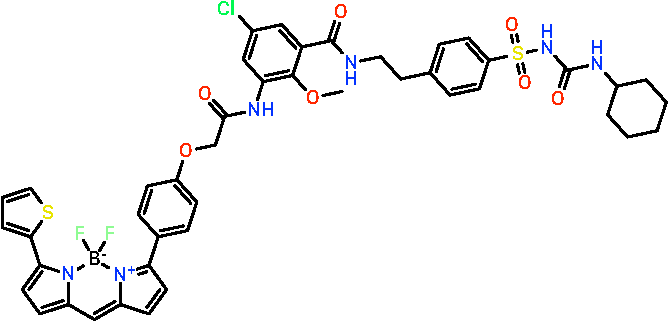
\includegraphics[width=\linewidth]{./Figuras/ER-Tracker_Blue.pdf}
		\caption{ER-Tracker™ Blue}
		\label{ER-Tracker_Blue}
	\end{subscheme}
	\hfill
	\begin{subscheme}{0.45\linewidth}
		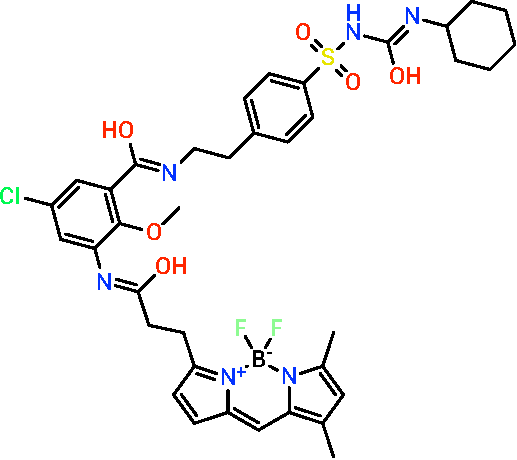
\includegraphics[width=\linewidth]{./Figuras/ER-Tracker_Green.pdf}
		\caption{ER-Tracker™ Green}
		\label{ER-Tracker_Green}
	\end{subscheme}
	\caption[ER-Trackers™]{Los ER-Tracker™ Green y ER-Tracker™ Red de Thermo Fischer Scientific™ son \gls{BODIPY} comerciales utilizados como agentes para la tinción celular.}
	\label{ER-Trackers}
\end{scheme}

Los \gls{FMR} son fluoróforos sensibles a la viscosidad que presentan una rotación libre que se vuelven fluorescentes, o en su defecto, aumentan la fluorescencia solo si su rotación se ve restringida. Algunas interacciones de carácter intramolecular para detener la rotación de los \gls{FMR} son \begin{inparaenum}[i.]
	\item formar interacciones de hidrógeno,\autocite{wuMultistageRotationalSpeed2018}
	\item a través del impedimento estérico,\autocite{faulknerAllostericRegulationRotational2016} o
	\item por la formación de complejos estables con iones metálicos.\autocite{yadavViscochromicMechanochromicUnsymmetrical2019}
\end{inparaenum}

Se ha determinado que la polaridad del solvente y la viscosidad del mismo afectan considerablemente la fluorescencia de los \gls{FMR}. Esto es porque se limita la tasa de formación del complejo \gls{TICT}, el cual se de-exita de forma \emph{no-radiativa,} y se promueve la formación del complejo \gls{LE}, el cual fluórese. El efecto que tiene la polaridad del solvente, aunque se sabe que es importante, no se ha logrado elucidar de forma aislada a la viscosidad.\cite{haidekkerEffectsSolventPolarity2005}

Diferentes estrategias para el diseño de \gls{FMR} se han propuesto para realizar sensores de viscosidad altamente sensibles, por ejemplo, incorporando grupos rotacionales asimétricos,\autocite{leePyrrolicMolecularRotors2016} usando grupos con alta capacidad para rotar,\autocite{karpenkoPushPullDioxaborine2016} variación de puentes π-conjugados del tipo \emph{push-pull},\autocite{karpenkoPushPullDioxaborine2016} la aplicación de rotadores di— o trímeros,\autocite{kimballBODIPYBODIPYDyad2015} y la introducción de dos rotadores distintos con diferentes capacidades rotacionales y electrodonadoras. \autocite{rautTriazinebasedBODIPYTrimer2016}

Por lo que, obtener tanto una alta eficiencia de fluorescencia como un contraste fluorescente simultáneamente es muy difícil, debido a que, en muchos casos, las moléculas de alto rendimiento cuántico tienen una capacidad de contraste deficiente.
El rendimiento cuántico y el contraste de fluorescencia de los \gls{FMR} están inversamente correlacionados, una relación llamada ``intensidad de fluorescencia---contraste".\autocite{leeFrontCoverFluorescent2018}

En la actualidad existe una amplia variedad de \gls{FMR} derivados de compuestos de boro, donde los \gls{BODIPY} y los dioxaborinos son los protagonistas debido a su elevado rendimiento cuántico, sin embargo, muestran algunas desventajas como la síntesis en varias etapas, condiciones de atmósfera anhidra y, en muchas ocasiones, una capacidad de contraste baja, aumentando escasamente el rendimiento cuántico del valor inicial.\autocite{karpenkoPushPullDioxaborine2016,guptaBodipyBasedFluorescent2016,liBODIPYBasedTwoPhotonFluorescent2018,kimBorondifluorideComplexesHemicurcuminoids2016}

Recientemente, nuestro grupo de trabajo ha informado sobre la síntesis de \gls{BOSCHIBA} y su uso como \gls{FMR} en la detección de viscosidad y la bioimagen de células.\autocite{ibarra-rodriguezFluorescentMolecularRotors2017} Los resultados encontrados indican que los \gls{BOSCHIBA} pueden aumentar hasta 34 veces su valor de rendimiento cuántico en medios de alta viscosidad, sin embargo, a pesar de teñir selectivamente el citoplasma en las células de melanoma, presentaron un bajo teñido atribuido principalmente a la baja solubilidad de los compuestos.

% Para lograr mejorar el contraste de fluorescencia y la bioimagen celular, se diseñó una serie de \gls{BOSCHIBA} derivados de aminoácidos (ver \cref{sch:marcha}), donde las moléculas presentan rotación libre a través del anillo fenilborónico, y el aminoácido podría dar una mayor compatibilidad y solubilidad en medios celulares.

Con el propósito de mejorar el contraste de fluorescencia y la bioimagen celular, se diseñó una serie de \gls{BOSCHIBA} derivados de aminoácidos (ver \cref{sch:marcha}). Estas \gls{BOSCHIBA} están diseñadas de tal manera que presenten una rotación libre a través del anillo fenilborónico, y se espera que los aminoácidos que se incorporarán a la estructura podrían resultar en una mayor permeabilidad de membranas celulares. Los compuestos de boro fluorescentes \reactant{BO-gly}, \reactant{BO-trp}, \reactant{BO-tyr} y \reactant{BO-phe} se sintetizarán por una reacción multicomponente en \gls{MW} con el objetivo de tener altos rendimientos químicos en un tiempo de reacción corto. Este método resulta más eficiente y rápido en comparación con \gls{BOSCHIBA} similares reportadas en la literatura, producidos por métodos convencionales.

\begin{scheme}[H]
	\centering
	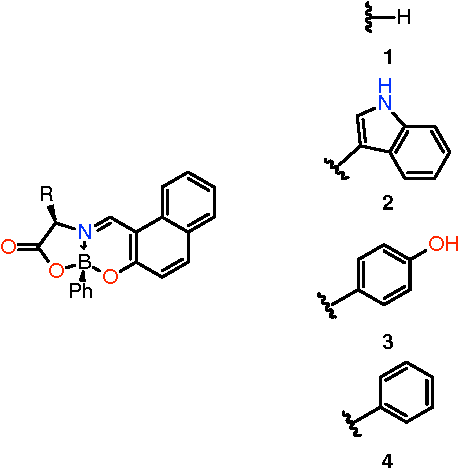
\includegraphics[width=0.5\linewidth]{./Figuras/Marcha.pdf}
	\caption{Compuestos que se sintetizarán en esta investigación.}
	\label{sch:marcha}
\end{scheme}